\section{Auswertung}
\label{sec:Auswertung}
Alle in der Auswertung benutzten Mittelwerte werden über die Gleichung
\begin{equation}
\tilde{x}=\frac{1}{n}\sum_{i=1}^n {x_i}
\end{equation}
bestimmt. Die Standardabweichung der Mittelwerte ergibt sich zu 
\begin{equation}
\Delta{\tilde{x}}=\sqrt{\frac{1}{n(n-1)}\sum_{i=1}^n {(x_i-\tilde{x})²}}.
\end{equation}
Wird eine Größe bestimmt, welche sich aus fehlerbehafteten Daten zusammensetzt, ergibt sich der absolute Fehler über die Gausssche Fehlerfortpflanzung 
\begin{equation}
\Delta{f}(x_1,..,x_n)=\sqrt{\left(\frac{\mathup{d}f}{\mathup{d}x_1}\Delta{x_1}\right)²+..+\left(\frac{\mathup{d}f}{\mathup{d}x_n}\Delta{x_n}\right)²}.
\end{equation}
Zur Berechnung aller Größen werden die nicht gerundeten Größen benutzt um Rundungsfehler zu vermeiden. Am Ende der Auswertung aller Größen werden diese auf die erste signifikante Stelle des Fehlers gerundet. 

\subsection{Bestimmung von \texorpdfstring{$\mu$}{Absorptionskoeffizient} und \texorpdfstring{$N_0$}{Anfangswert} für Blei und Eisen mit Hilfe von \texorpdfstring{$\gamma$}{Gamma}-Strahlung}
Der Nulleffekt für beide Messungen ergibt sich durch den Quotienten der gemessenen Zerfälle $n$ pro Zeiteinheit ${\mathup{\Delta{t}}}$ zu
\begin{equation}
N_\mathup{u}=\frac{n}{\mathup{\Delta{t}}}=\frac{682}{\SI{750}{\second}}=0,91\,\frac{1}{\si\second}.
\label{eq:N_u}
\end{equation}
Es werden der Absorptionskoeffizient $\mu$ und $N_0$ für Blei und Eisen bestimmt. Dabei werden die Materialien der Strahlung eines $\ce{^{137}Cs}$--Strahlers ausgesetzt. 
\begin{table}[p]
\begin{minipage}[t]{0.5\linewidth}
	\centering
	\sisetup{table-format=2.2}
\begin{tabular}{S[table-format=2.1] S[table-format=3.0] S[table-format=5.0] S[table-format=3.2]}
\toprule
{$d\:/\si{\milli\meter}$} & {$t\:/\si\second$} & {$n$} & {$N-N_\mathup{u}$}\\
\midrule
 1.2 &   80 & 10700 &  132.84\\
 1.3 &   80 & 10630 &  131.97\\
 2.4 &   80 &  8919 &   48.31\\
 6.0 &   80 &  6690 &   17.89\\
10.3 &  120 &  5906 &    5.89\\
12.9 &  120 &  4569 &  110.58\\
20.2 &  180 &  3383 &   14.42\\
21.4 &  120 &  1840 &   82.72\\
30.5 &  180 &  1223 &    1.96\\
40.4 &  180 &  516  &   37.17\\
		\bottomrule
	\end{tabular}
	\caption{Messwerte für Blei.}
\label{tab:werte_gamma_blei} 
\end{minipage}
\hfill
    \begin{minipage}[t]{0.5\linewidth}
	\centering
	\sisetup{table-format=2.2}
	\begin{tabular}{S[table-format=2.1] S[table-format=3.0] S[table-format=5.0] S[table-format=3.2]}
\toprule
{$d\:/\si{\milli\meter}$} & {$t\:/\si\second$} & {$n$} & {$N-N_\mathup{u}$}\\
\midrule
 0.5 &   80 & 11878 & 147.57\\
 1.5 &   80 & 11284 & 140.14\\
 3.0 &   80 & 10345 & 128.40\\
 5.0 &   80 &  9563 & 118.63\\
 5.0 &  120 &  8007 &  65.82\\
10.0 &  120 & 11095 &  91.55\\
20.0 &  120 &  6402 &  52.44\\
25.0 &  180 &  7622 &  41.44\\
30.0 &  180 &  5958 &  32.19\\
40.0 &  180 &  3254  & 17.17\\
\bottomrule
	\end{tabular}
	\caption{Messwerte für Eisen.}
\label{tab:werte_gamma_eisen}
\end{minipage}
\end{table}
In den Tabellen \ref{tab:werte_gamma_blei} und \ref{tab:werte_gamma_eisen} sind die Messwerte, sowie die um denn Nulleffekt $N_\mathup{u}$ korrigierten Intensitäten aufgetragen. 
Wird der Logarithmus der korrigierten Intensitäten, dargestellt in Tabelle \ref{tab:log_werte}, gegen die Schichtdicke $d$ aufgetragen, ergibt sich ein linearer Zusammenhang. 
\begin{table}
\centering
\begin{tabular}{S[table-format=2.1] S[table-format=3.0] S[table-format=5.0] S[table-format=3.2] S[table-format=1.2]}
\toprule
\multicolumn{2}{c}{$\ln{(N-N_\mathup{u})}$} \\
{Blei} & {Eisen}\\
\midrule
4.89 & 4.99\\
4.88 & 4.94\\
3.88 & 4.86\\
2.88 & 4.78\\
1.77 & 4.19\\
4.71 & 4.52\\
2.67 & 3.96\\
4.42 & 3.72\\
0.67 & 3.47\\
3.62 & 2.84\\
\bottomrule
\end{tabular}
\caption{Logarithmus der korrigierten Intensitäten für Blei und Eisen.}
\label{tab:log_werte}
\end{table}
\begin{figure}
	\centering
	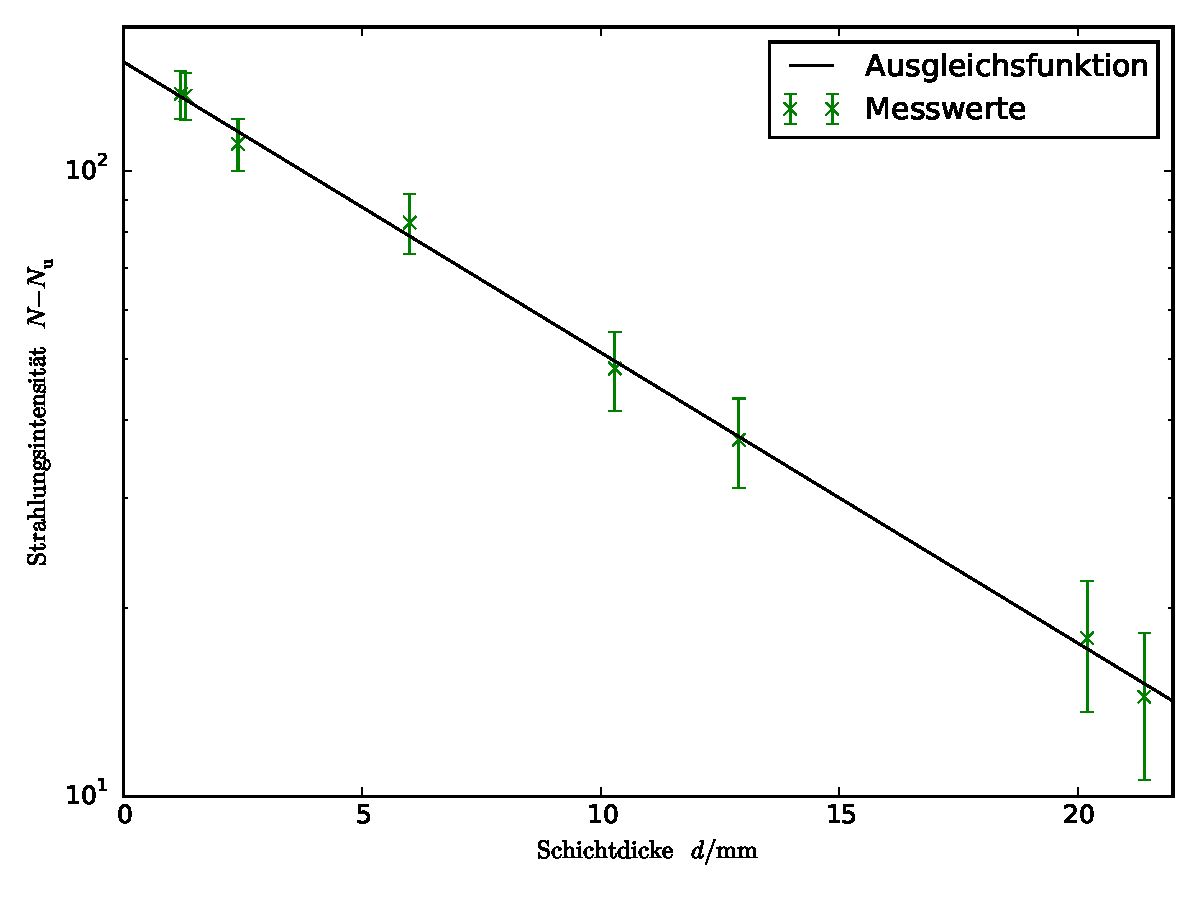
\includegraphics[width=0.9\textwidth]{Bilder/Blei.pdf}
	\caption{Schichtdicke $d$ aufgetragen gegen die Strahlungsintensität.}
	\label{fig:blei}
\end{figure}
\begin{figure}
	\centering
	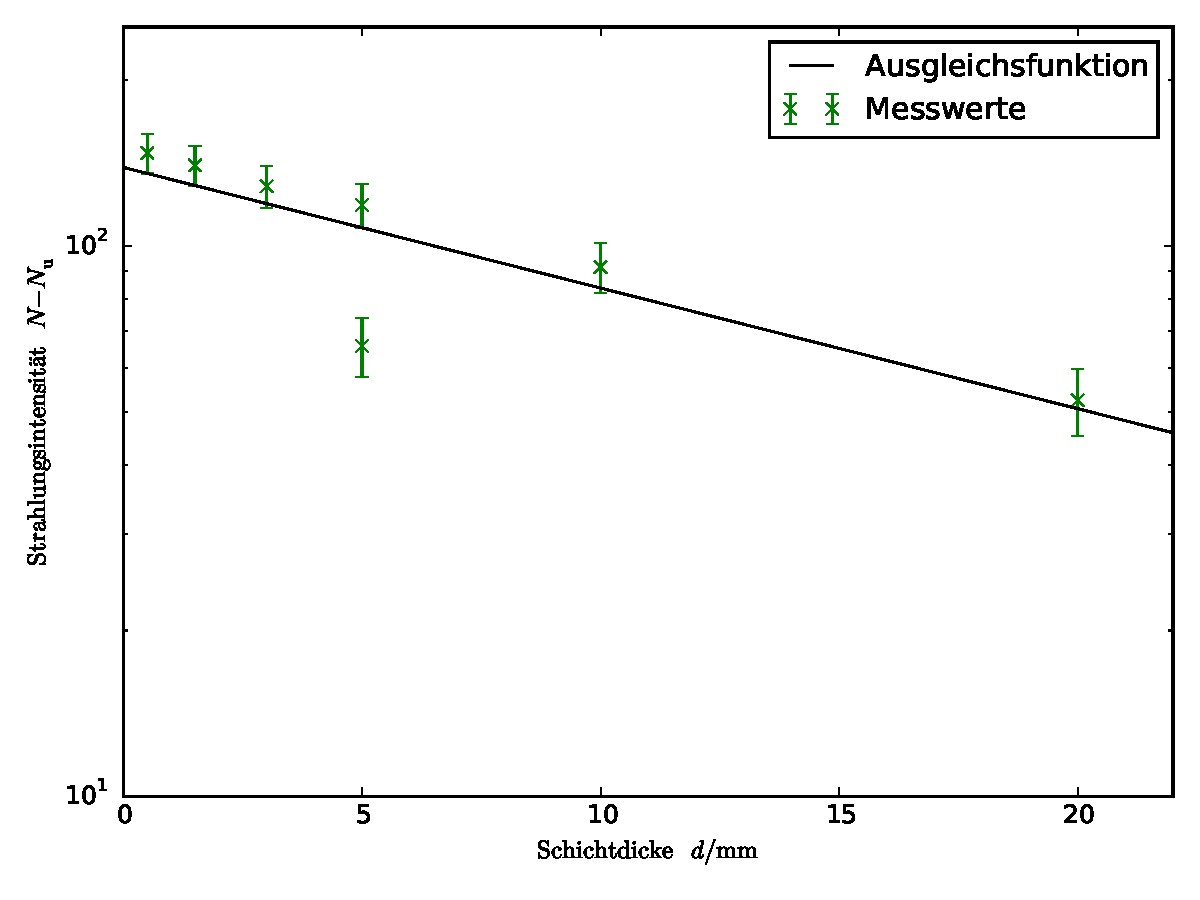
\includegraphics[width=0.9\textwidth]{Bilder/Eisen.pdf}
	\caption{Schichtdicke $d$ aufgetragen gegen die Strahlungsintensität.}
	\label{fig:eisen}
\end{figure}
Dieser ist samt Ausgleichsgerade für Blei in Abbildung \ref{fig:blei} und für Eisen in Abbildung \ref{fig:eisen} zu sehen.
Die lineare Regression ergibt die Geradengleichungen 
\begin{align}
f_\mathup{Pb}(x)&=(-107,0\pm0,9)x+(5,01\pm0,02),\\
f_\mathup{Fe}(x)&=(-50\pm5)x+(4,93\pm0,09).
\label{eq:lin_regress}
\end{align}
Aus ihnen lassen sich die gesuchten Größen $\mu$ und $N_0$ bestimmen. 
Die Absorptionskoeffizienten entsprechen der Steigung der Geraden; die Anfangswerte $N_0$ lassen sich nach Vergleich der Gleichungen \eqref{eq:Absorptionsgesetz_Vorstufe} und \eqref{eq:Absorptionsgesetz} berechnen.
Es ergeben sich die Absorptionskoeffizienten $\mu$ und $N_0$ zu
\begin{align}
\mu_\mathup{Pb}&=-(107,0\pm0,9)\,\frac{1}{\si\meter} &\text{und}\quad  N_{0\mathup{,Pb}}&=(150\pm1)\,\frac{1}{\si\second},\\
\mu_\mathup{Fe}&=-(50\pm5)\,\frac{1}{\si\meter}  &\text{und}\quad  N_{0\mathup{,Fe}}&=(138\pm1)\,\frac{1}{\si\second}.
\end{align}
Damit sind die Absorptionsgesetze
\begin{align}
N_\mathup{Pb}(d)&=(150\pm1)\,\frac{1}{\si\second}\cdot\mathup{e}^{-(107,0\pm0,9)\,\frac{1}{\si\meter}d},\\
N_\mathup{Fe}(d)&=(138\pm1)\,\frac{1}{\si\second}\cdot\mathup{e}^{-(50\pm5)\,\frac{1}{\si\meter}d}.
\end{align}
 für Blei und Eisen bestimmt.


\subsection{Vergleich von Theorie und Experiment}
Um die Ergebnisse der Untersuchung von Materie mit $\gamma$-Strahlung bewerten zu können werden der Absorptionskoeffizient $\mu_\mathup{C}$ über den Wirkungsquerschnitt $\sigma_\mathup{C}$  nach Compton bestimmt wie in der Theorie beschrieben. Verwendet werden dabei die charakteristische Größe $\epsilon=1,295$, sowie die in Tabelle \ref{tab:werte} aufgelisteten Größen.
\begin{table}
\centering
\begin{tabular}{S S[table-format=2.0] S[table-format=3.1] S[table-format=2.3]}
\toprule
{Material} & {$Z$} & {$M\:/\frac{\si\gram}{\si\mol}$} & {$\rho\:/\frac{\si\gram}{\si{\centi\meter}^3}$}\\
\midrule
\text{Blei} & 82 & 207.2 & 11.342\\
\text{Eisen} &26 & 55.8  & 7.874\\
\bottomrule
\end{tabular}
\caption{Materialkonstanten, benötigt zur Berechnung von $\mu_\mathup{C}$ für Blei und Eisen.}
\label{tab:werte}
\end{table}
Mit Gleichung \eqref{eq:sigma_c} ergeben sich für die Wirkungsquerschnitte
\begin{equation}
\mu_\mathup{C,Pb}=\mu_\mathup{C,Fe}=2,57\cdot10^{-29}
\end{equation}
und daraus resultierend die Absorptionskoeffizienten
\begin{equation}
\mu_\mathup{C,Pb}=69,43\,\frac{1}{\si\meter} \quad\text{und}\quad \mu_\mathup{C,Fe}=56,76\,\frac{1}{\si\meter}.
\end{equation}
Der Absorptionskoeffizient von Eisen weicht um $54,11\%$ von der Theorie ab. Dieser große Unterschied zeigt auf, dass die Compton-Streuung nur eine geringe Rolle spielt und der Photoeffekt mehr Einfluss besitzt. Blei, mit einer Abweichung von $11,91\%$, wechselwirkt mit der Strahlung hauptsächlich über Compton-Streuung. Der Photoeffekt spielt hier nur eine kleine Rolle. Da die Energien niedrig sind, kann die Paarerzeugung als Wechselwirkungsprozess fast vollkommen ausgeschlossen werden.
\subsection{Maximale Energie der Strahlung}
Erneut wird der Nulleffekt $N_\mathup{u}$ nach Gleichung \eqref{eq:N_u} zu
\begin{equation}
N_\mathup{u}=\frac{273}{\SI{750}{\second}}=0,364\,\frac{1}{\si\second}
\end{equation}
bestimmt. 

\begin{table}
\centering
\begin{tabular}{S[table-format=3.1(2)] S[table-format=3.0] S[table-format=5.0] S[table-format=2.3]}
\toprule
{$d\:/\si{\micro\meter}$} & {$t\:/\si\second$} & {$n$} & {$N-N_u$}\\
\midrule
102(1)   & 350 &18401 & 52.210\\
126(1)   & 350 & 8934 & 25.516\\
153.0(5) & 350 & 3693 & 10.187\\
160(1)   & 350 & 2230 &  6.007\\
200(1)   & 350 &  736 &  1.739\\
253(1)   & 350 &  225 &  0.279\\
302(1)   & 500 &  199 &  0.034\\
338(5)   & 500 &  187 &  0.010\\
400(1)   & 500 &  211 &  0.058\\
444(2)   & 500 &  271 &  0.178\\
\bottomrule
\end{tabular}
\caption{Messwerte der unterschiedlichen Absorberdicken.}
\label{tab:werte_beta}
\end{table}
Wird die Intensität halblogarithmisch gegen die Schichtdicke aufgetragen kann die maximale Reichweite $R_\mathup{max}$ der $\beta$-Teilchen durch den Schnitt zweier Geraden. Die erste Gerade
\begin{equation}
g_1(x)=\underbrace{-(35000\pm2000)}_{\text{Steigung} m_1}x+\underbrace{(7,6\pm0,3)}_{y-\text{Achsen}-\text{Abschnitt} b_1}
\end{equation}
ergibt sich durch die Regression der Werte 1 bis 6; die zweite Gerade
\begin{equation}
g_2(x)=\underbrace{-(2,8\pm0,6)}_{y-\text{Achsen}-\text{Abschnitt} b_2}
\end{equation}
aus den restlichen Werten.Wird $m_2$ durch lineare Regression bestimmt ergbit sich ein Fehler, der ein Vielfaches des Wertes selbst und damit unbrauchbar ist.Daher besitzt Gerade $2$ die Steigung $m_2=0$; nur der $y$-Achsen-Abschnitt wird durch die Ausgleichsrechnung bestimmt. 
Der Schnitt kann berechnet werden über 
\begin{equation}
R_\mathup{max}=\frac{b_2-b_1}{m_2-m_1}.
\end{equation}
Nach Gleichung \eqref{eq:e_max} kann daraus die maximale Energie bestimmt werden. Damit ergeben sich die maximale Reichweite und die maximale Energie der untersuchten $\beta$-Strahlung zu
\begin{align}
R_\mathup{max}=(29\pm2)\,\si\meter \quad\text{und}\quad E_\mathup{max}=(0,30\pm0,07)\,\mathup{e}\si\volt
\end{align}
\begin{figure}
	\centering
	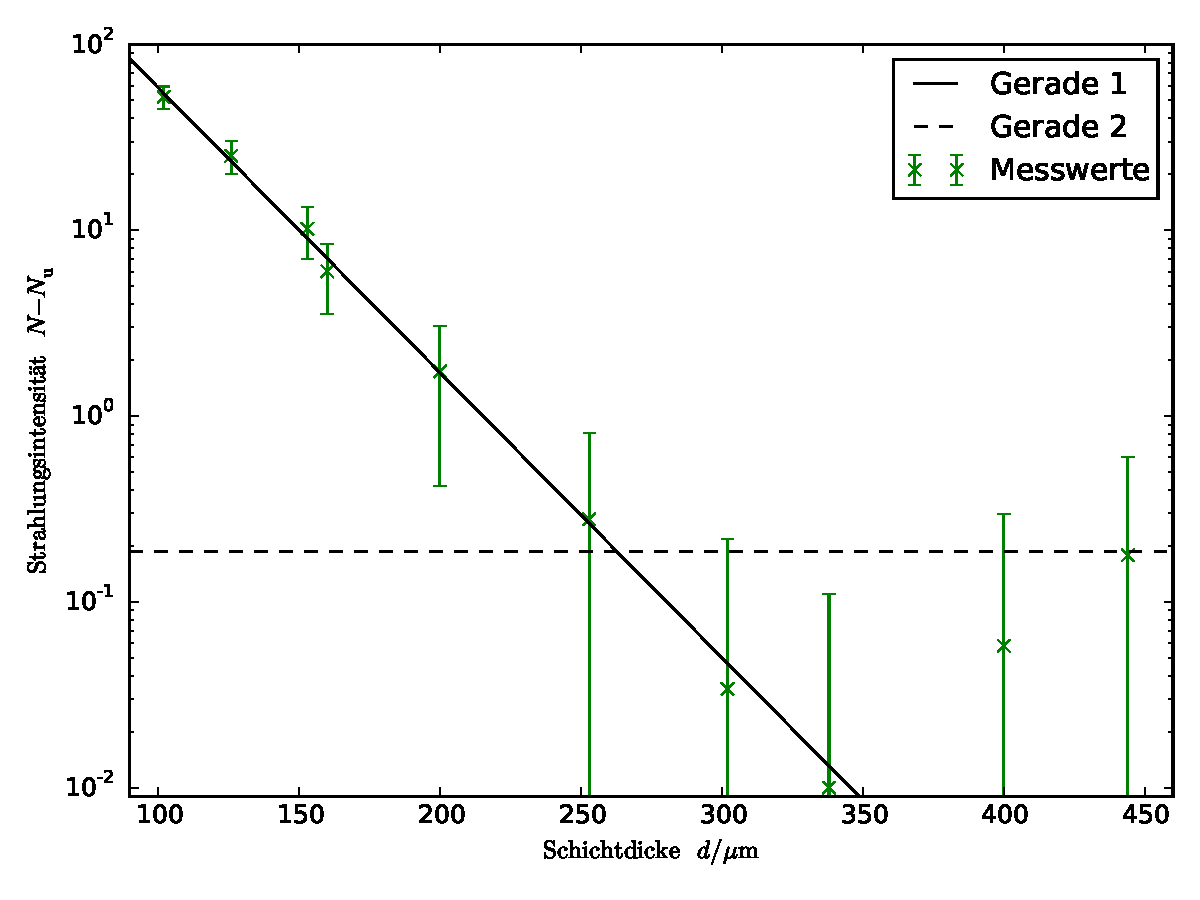
\includegraphics[width=0.9\textwidth]{Bilder/beta.pdf}
	\caption{Reichweite des Schallimpulses in Abhängigkeit von der Laufzeit, Regression zur Bestimmung der Geschwindigkeit.}
	\label{fig:geschwindigkeit}
\end{figure}


